% template.tex, dated April 5 2013
% This is a template file for Annual Reviews 1 column Journals
%
% Compilation using ar-1col.cls' - version 1.0, Aptara Inc.
% (c) 2013 AR
%
% Steps to compile: latex latex latex
%
% For tracking purposes => this is v1.0 - Apr. 2013

\documentclass{ar-1col}
\usepackage{url}
\usepackage[numbers,sort&compress]{natbib}

%% added packages
\usepackage{xspace}
\usepackage{graphicx}
\usepackage{amssymb}
%\usepackage[top=2cm,bottom=3cm]{geometry}
\usepackage[svgnames]{xcolor}
% hyper-ref prevents the document from compiling on the arXiv - it is
% included in some other `usepackage` and that generates a conflict.
% Will attempt to use it differently, hope for a better outcome.
%\usepackage[bookmarks=false]{hyperref}
\usepackage[bookmarks=false,colorlinks=true,linkcolor=DarkBlue,citecolor=DarkBlue]{hyperref}
\usepackage{subfig}
%\usepackage{subcaption}
\usepackage{rotating}
\usepackage{units}
\usepackage{amsmath}
\usepackage{bm}     % nice math bold italics
\usepackage{lineno}
\usepackage{listings}
\usepackage{lmodern} % suppress font warnings
\usepackage[normalem]{ulem}
\usepackage[section]{placeins}
\usepackage{hepunits}
\usepackage{hepparticles}
\usepackage{cancel}
\usepackage{hepnames}
%\usepackage{epstopdf}
\usepackage{mathtools}
\usepackage[capitalise]{cleveref}
\usepackage{braket}
\usepackage{slashed}
\usepackage{xcolor}
\usepackage{multirow}

\usepackage[Export]{adjustbox}

% Greek letters
\def\g{\gamma}
\def\t{\tau}

\def\D{\Delta}
\def\G{\Gamma}
\def\O{\Omega}

% math
\makeatletter
\newcommand*\dotp{\mathpalette\bigcdot@{.5}}
\newcommand*\bigcdot@[2]{\mathbin{\vcenter{\hbox{\scalebox{#2}{$\m@th#1\bullet$}}}}}
\makeatother


\def\Dslash{D\hskip-0.65em /}
\def\tsep{t_{\rm sep}}
\def\tmin{t_{\rm min}}


%\newcommand{\Umunu}{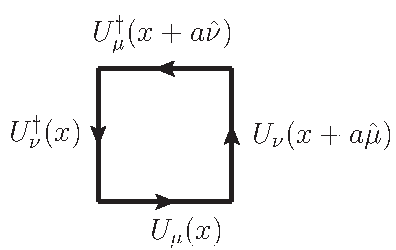
\includegraphics[width=0.5\textwidth,fbox=1pt,valign=c]{plots/plaquette}}
\newcommand{\Umunu}{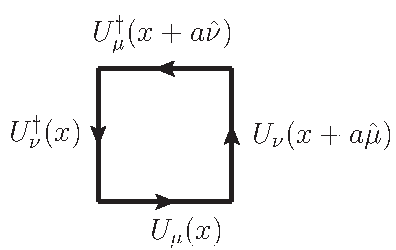
\includegraphics[width=0.6\textwidth,valign=c]{plots/plaquette}}

\setcounter{secnumdepth}{4}
\def\addcite#1{{\color{red}CITE[#1]}}
\def\addcomment#1{{\color{red}COMMENT: #1}}
\def\new#1{{\color{blue}#1}}
\def\asm#1{{\color{red}#1}}
\def\done#1{{\color{gray}#1}}


% Metadata Information
\jname{Xxxx. Xxx. Xxx. Xxx.}
\jvol{AA}
\jyear{2022}
\doi{10.1146/((please add article doi))}


% Document starts
\begin{document}

% Page header
\markboth{A. Meyer, A. Walker-Loud, C. Wilkinson}{LQCD relevance for the few-GeV neutrino program}

% Title
\title{Status of Lattice QCD Determination of Nucleon Form Factors
 and their Relevance for the Few-GeV Neutrino Program}

%Authors, affiliations address.
\author{Aaron S. Meyer$^1$,
Andr\'{e} Walker-Loud$^2$,
Callum Wilkinson$^3$
\affil{$^1$Department of Physics, University of California, Berkeley, CA, 94720, USA}
\affil{$^2$Nuclear Science Division, Lawrence Berkeley National Laboratory, Berkeley, CA, 94720, USA}
\affil{$^3$Physics Division, Lawrence Berkeley National Laboratory, Berkeley, CA, 94720, USA}
}

\begin{abstract}
  ...
\end{abstract}

%Keywords, etc.
\begin{keywords}
Neutrino Oscillations, Nucleon Form Factors, Lattice QCD
%keywords, separated by comma, no full stop, lowercase
\end{keywords}

\maketitle

%Table of Contents
\tableofcontents


% ------------------------------------------------------------------------------
% Intoroduction
\section{Introduction\label{sec:intro}}
A major experimental program is underway which seeks to measure
as of yet unknown properties associated with the change of flavor of neutrinos.
In particular, the neutrino mass hierarchy and%
\begin{marginnote}
\entry{CP}{charge-parity}
\end{marginnote}%
CP violating phase
of neutrinos still remain to be measured, with additional focuses on measuring
oscillation parameters with high precision and testing whether the current
three-flavor mixing paradigm is sufficient~\cite{Esteban:2020cvm, ParticleDataGroup:2020ssz}.
These goals introduce stringent requirements on the precision of current and future experiments.
High-intensity beams are required to produce the flux of neutrinos to be able to accumulate the necessary statistics.
Increased statistics place additional burden on our understanding of the systematic uncertainties needed for the experimental program.


Two, billion dollar scale, next-generation experiments designed to meet these experimental constraints
are
%the Deep Underground Neutrino Experiment (DUNE)~\cite{Abi:2020wmh}
DUNE~\cite{Abi:2020wmh}
and the
%Hyper-Kamiokande experiment (Hyper-K)~\cite{Hyper-Kamiokande:2018ofw}.
Hyper-K experiment~\cite{Hyper-Kamiokande:2018ofw}.
DUNE has a broad neutrino energy spectrum with a peak at a neutrino energy of $\approx$2.5 GeV,
but significant contributions between 0.1--10 GeV, over a 1295 km baseline.
Hyper-K has a narrow neutrino energy spectrum peaked at a neutrino energy of $\approx$0.6 GeV, with significant
contributions between 0.1--2 GeV, over a 295 km baseline. Despite their different energies (E) and
baselines (L), both experiments sit at a similar L/E, so probe similar oscillation physics.%
%-------------------------------------------------------------------------------
\begin{marginnote}
    \entry{DUNE}{Deep Underground Neutrino Experiment}
    \entry{Hyper-K}{Hyper Kamiokande}
\end{marginnote}%
%-------------------------------------------------------------------------------
At the few-GeV energies of interest, neutrino interactions with nucleons have many available interaction channels,
including quasielastic, resonant, and deep inelastic scattering~\cite{zeller12, hayato_review_2014, Mosel:2016cwa, Katori:2016yel, NuSTEC:2017hzk}.
All current and planned experiments use nuclear targets ($^{12}$C--$^{40}$Ar) as the
target material to increase the interaction rate, as well as to avoid serious experimental complications using elementary targets.
The use of nuclear targets significantly complicates the cross-section modeling issues and
associated systematics as intra-nuclear dynamics have a comparable energy scale to
the energy transfers in the neutrino interactions of interest.

A significant challenge impeding progress towards a consistent theoretical description of neutrino-nucleus interactions is the lack of data to benchmark parts of the calculation against. For example, neutrino quasielastic scattering ($\nu_{l} + n \rightarrow l^{-} + p$ or $\bar{\nu}_{l} + p \rightarrow l^{+} + n$) is the simplest of the relevant hard scattering processes, and dominates the neutrino cross section below energies of $\approx$1 GeV. However, modern experiments using nuclear targets are unable to measure it without significant nuclear effects~\cite{garvey_review_2014, NuSTEC:2017hzk}.
Neutrino cross-section models for quasielastic scattering (and other hard-scattering processes) have relied heavily on sparse data from the 1960--1980's from several bubble chamber experiments which used H$_{2}$ or D$_2$ targets~\cite{zeller12, ParticleDataGroup:2020ssz}.
The small neutrino cross section, and relatively weak (by modern standards) accelerator neutrino beams utilized by these early experiments, mean that the available quasielastic event sample on light targets amounts to a few thousand events~\cite{ANL_Barish_1977, BNL_Fanourakis_1980, BNL_Baker_1981, Kitagaki:1983px, Allasia:1990uy}.%
\footnote{Some constraints on the axial form factor have been obtained from fits
 to pion electroproduction data.
The fits are parameterized by a low energy theory that is valid in the chiral
 ($m_\pi\to0$) limit and close to threshold.
These data will be ignored in this review.
For more details, we refer the reader to Refs.~\cite{Bernard:1993bq,Bernard:2001rs}.
}

The sparse data from deuterium bubble-chamber experiments do not constrain
the axial form factor precisely.
The popular dipole ansatz has a shape that
is overconstrained by data resulting in an underestimated uncertainty.
Employing a model-independent $z$-expansion parameterization
relaxes the strict shape requirements of the dipole and yields
a more realistic uncertainty that is nearly an order of magnitude larger~\cite{Meyer:2016oeg}.
The axial radius, which is proportional to the slope of the form factor at $Q^2=0$,
has a 50\% uncertainty when estimated from the deuterium scattering data,
or $\approx35\%$ if deuterium scattering and muonic hydrogen are considered
together~\cite{Hill:2017wgb}.
Ideally, the lack of precision in the axial form factor would
be rectified by a modern neutrino-scattering experiment.

Safety considerations make it unlikely that new high-statistics bubble-chamber experiments using
hydrogen or deuterium will be deployed to fill this crucial gap,
so experimentalists are looking for other ways to access neutrino interactions
with elementary targets as a tool for disambiguating neutrino cross-section modeling uncertainties.
One possibility is to use various hydrocarbon targets to subtract the carbon interaction contributions from
the total hydrocarbon event rates, and produce ``on hydrogen'' measurements~\cite{PhysRevD.92.051302, PhysRevD.101.092003, Hamacher-Baumann:2020ogq, DUNE:2021tad}.
These ideas are promising, but typically rely on kinematic tricks that are only relevant for some channels, and it remains to be seen whether the systematic uncertainty associated with modeling the carbon subtraction can be adequately controlled. Such ideas may also be extended to other compound target materials with hydrogen or deuterium components.

In the absence of such an updated experiment,%
\begin{marginnote}
\entry{LQCD}{Lattice quantum chromodynamics}
\end{marginnote}%
LQCD can provide the missing free nucleon amplitudes
that are otherwise not known at the required precision.
LQCD provides a theoretical alternative for predicting the free nucleon amplitudes directly from the Standard Model of particle physics, with systematically improvable theoretical uncertainties.
Recently, a benchmark LQCD calculation was achieved in which the nucleon axial charge (the axial form factor at zero momentum transfer) was determined with a 1\% total uncertainty~\cite{Chang:2018uxx}.
LQCD can also provide percent to few-percent level uncertainties for the nucleon quasielastic axial form factor with a few-${\rm GeV}^2$ reach in momentum transfer.
Similarly, current tension in the neutron magnetic form factor parameterization, which is roughly half the size of the total axial form factor uncertainty, can be resolved with LQCD calculations.
Such results are anticipated in the next year or so with computing power available in the present near-exascale computing era.

Building upon these critical quantities, more challenging computations can provide information about nucleon
resonant and nonresonant contributions to vector and axial-vector matrix elements,
such as the $\Delta$ or Roper resonance channels, pion-production,
inclusive contributions in the shallow inelastic scattering region,
or deep inelastic scattering parton distribution functions.
Additionally, two-nucleon response functions can be computed which can provide crucial information for our theoretical understanding of important two-body currents which are needed for understanding the neutrino-nucleus cross sections.


Given the present state of the field, in this review, we focus on elastic single-nucleon amplitudes, in which we anticipate the LQCD results will become impactful for the experimental programs in the next year or two.
We begin in Section~\ref{sec:sof} by surveying the existing status and tension in the field for the single-nucleon (quasi-) elastic form factors.
Then, in Section~\ref{sec:lqcd}, after providing a high-level introduction to LQCD, we survey existing results of the axial form factor including the role of the%
\begin{marginnote}
 \entry{PCAC} {Partially-conserved} axial current
\end{marginnote}%
PCAC relation in the calculations as well as use of the $z$-expansion for combining the continuum and physical pion mass extrapolations.
In Section~\ref{sec:impact}, we discuss the potential impact of using LQCD determinations of the axial form factor when modeling neutrino-nucleus cross sections.
In Section~\ref{sec:future}, we comment on the most important improvements to be made in LQCD calculations and we conclude in Section~\ref{sec:conclusions}.



%-------------------------------------------------------------------------------
% State of the field
\section{Status of single nucleon (quasi-) elastic form factors\label{sec:sof}}
For charged current quasielastic $\nu N$ scattering,
the neutron ($|n\rangle$) to proton ($\langle p|$)
interaction is described by a $V-A$ weak interaction, given at the quark level by
$\bar{u}\gamma_\mu(1- \gamma_5)d$ (or its conjugate for proton to neutron), with the nucleon level amplitude at four-momentum transfer $Q^2 = -q^2$ parameterized by
\begin{align}\label{eq:nucleon_ff}
\langle p | V^\mu | n \rangle
    &= \bar{U}_p(p+q) \Big[
        F_1^+(q^2) \gamma^\mu
        +\frac{i}{2M} F_2^+(q^2) \sigma^{\mu\nu} q_\nu
    \Big] U_n(p),
\nonumber\\
\langle p | A^\mu | n \rangle
    &= \bar{U}_p(p+q) \Big[
        F_{\mathrm{A}}^+(q^2) \gamma^\mu \gamma_5
        +\frac{1}{M} F_P^+(q^2) q^\mu \gamma_5
    \Big] U_n(p)\, .
\end{align}
The isovector, vector form factors, $F_1^+$ and $F_2^+$, can be precisely estimated from electron-nucleon scattering data.
Electron-proton and electron-neutron scattering are sensitive to the isoscalar, $F_{1,2}^s$ and isovector, $F_{1,2}^3$ form factors.  After isolating $F_{1,2}^3$, approximate isospin symmetry can be used to relate these $\tau_3$ form factors to the charged $\tau_+$ form factors of Equation~\eqref{eq:nucleon_ff}: in the isospin limit, $\langle p| \bar{u}\, \Gamma u - \bar{d}\, \Gamma d |p\rangle = \langle p| \bar{u}\, \Gamma d |n\rangle$
 for Dirac structure $\Gamma$ \new{and $F_{1,2}^3 = F_{1,2}^+$
 for the isovector Dirac and Pauli form factors}.
%The overall uncertainty of the electron-neutron form factors is larger than those of the proton due to the relative sparsity of electron-neutron data.
%------------------------------------------------------------------------------
% proton magnetic FF
\begin{figure}
 \centering
 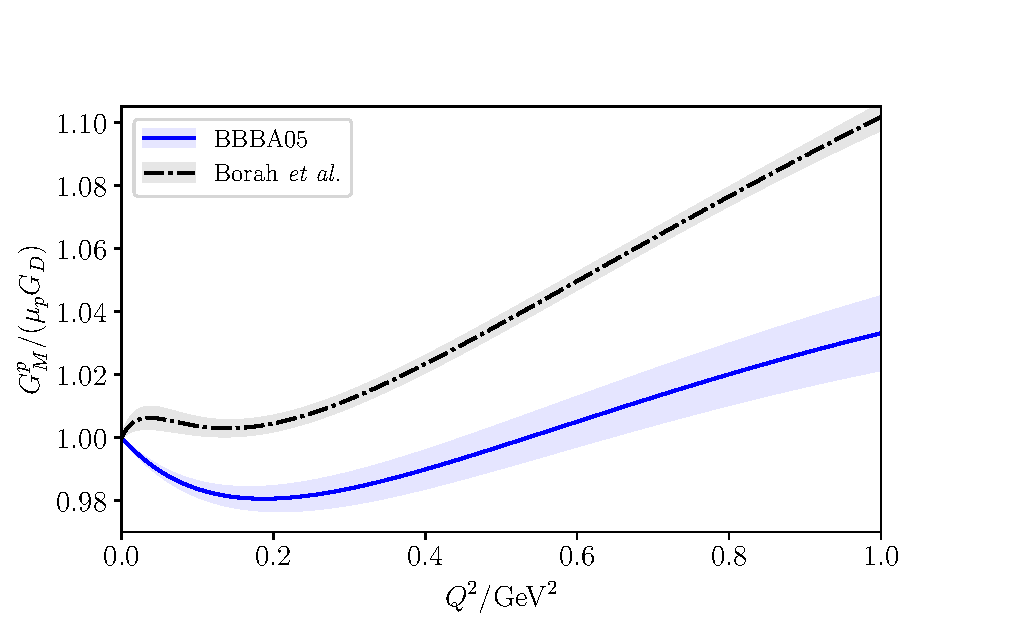
\includegraphics[width=0.7\textwidth]{plots/proton_magnetic-standalone.pdf}
 \vspace{4pt}
\caption{
Proton magnetic form factor normalized by a reference dipole ansatz
with a dipole mass of $0.84~{\rm GeV}$.
This plot is reproduced from Fig.~4 in Ref.~\cite{Borah:2020gte}
 and the associated supplemental data.
The proton-only fit to a $z$-expansion by Borah {\it et al.}~\cite{Borah:2020gte}
and the BBBA05 parameterization~\cite{Bradford:2006yz} are shown.
\label{fig:protonmagneticff}
}
\end{figure}
%------------------------------------------------------------------------------

However, there is a significant tension in existing parameterizations of the proton magnetic form factor, as
shown in Figure~\ref{fig:protonmagneticff}.
Two different parameterizations of the form factor, normalized by the dipole, are shown.%
\begin{marginnote}
\entry{BBBA05}{The Bradford, Bodek, Budd and Arrington 2005 nucleon elastic form factor parameterization~\cite{Bradford:2006yz}}
\end{marginnote}%
The BBBA05~\cite{Bradford:2006yz} are displayed as the lower (blue) band with a solid mean value.
A more recent $z$-expansion parameterization from Borah {\it et al.}~\cite{Borah:2020gte} is displayed by the upper (black) band with a dashed mean value.
The tension is significant over all $Q^2 > 0$, at the level of several percent,
including significant disagreement in the slope of the form factor at $Q^2 = 0$.
Of the nucleon form factor calculations from LQCD,
the vector form factors are also the most mature,
exhibiting no obvious tensions with experimental determinations
of the vector form factors at their current level of precision.
A percent level calculation of the form factor $Q^2$ behavior combined with a direct calculation of the slope of the magnetic form factor would provide useful insight about this tension or could discriminate
between the two parameterizations.

The nucleon axial form factor has had a much more complicated past than the vector form factors in LQCD.%
\begin{marginnote}
 \entry{Axial charge} {The axial form factor at zero momentum transfer, $g_{\mathrm{A}} = F_{\mathrm{A}}(0)$}
\end{marginnote}%
The axial charge is a key benchmark for LQCD and is precisely known
from neutron decay experiments~\cite{Dubbers:2021wqv}.
LQCD calculations of the axial charge have historically been low compared to experiment~\cite{Aoki:2021kgd},
 and the discrepancy has been the topic of some controversy.
It is now understood that the treatment of excited state systematics is the main culprit for this discrepancy~\cite{Bar:2017kxh,Ottnad:2020qbw,Aoki:2021kgd}.
With proper control over the excited state contamination, the LQCD calculations are now in good agreement with the experimental value~\cite{Jang:2019vkm,Gupta:2018qil,Alexandrou:2020okk,Abramczyk:2019fnf,Park:2021ypf,RQCD:2019jai,Hasan:2019noy,Djukanovic:2021yqg,Harris:2019bih,Liang:2018pis,Shintani:2018ozy,Ishikawa:2018rew}
 with one group achieving a sub-percent determination of $g_{\mathrm{A}}$~\cite{Chang:2018uxx,Berkowitz:2018gqe,Walker-Loud:2019cif}.

Armed with the newfound confidence in the control of systematics for the axial charge,
 more emphasis is now being put into the form factor at nonzero momentum transfer
to make contact with the needs of the neutrino community and provide
 complementary constraints on free nucleon amplitudes.
One extremely striking feature of LQCD calculations is the strong preference for a slower
fall off of the form factor with increasing $Q^2$ than predicted by phenomenological determinations from experiment (Figure~\ref{fig:gaq2_overlay}).
This preference is consistently reproduced by several lattice collaborations using
independent computation methods, lending more credence to the result.
When integrated over the full range of $Q^2$ to compute the nucleon cross section,
this translates to an enhancement in the free nucleon cross section as large as 30--40\%
over neutrino energies greater than $1~{\rm GeV}$ (Section~\ref{sec:impact}).
In addition, the precision on the axial form factor uncertainty from LQCD
is small enough to be sensitive to the tension between vector form factor parameterizations.

The aforementioned situation with nucleon form factors is depicted in Figure~\ref{fig:nucleonxsec}.
The labels correspond to the following form factor parameterization choices and uncertainties:
\begin{description}
 \item[BBBA05] Vector form factors from BBBA05~\cite{Bradford:2006yz},
 and axial form factors from Meyer~{\it et al.}~\cite{Meyer:2016oeg}.
 The uncertainty is taken from BBBA05, with all fit parameters assumed to be uncorrelated.
 \item[$z$ exp, vector] Vector form factors from Borah~{\it et al.}~\cite{Borah:2020gte},
 and axial form factors from Meyer~{\it et al.}~\cite{Meyer:2016oeg}.
 The uncertainty is taken from Borah~{\it et al.}
 \item[$z$ exp, ${\rm D}_{2}$ axial] as ``$z$ exp, vector,''
 with the uncertainty taken from Meyer~{\it et al.} instead.
 \item[$z$ exp, LQCD axial] Vector form factors from Borah~{\it et al.}~\cite{Borah:2020gte},
 axial form factors and their uncertainty provided by authors from an LQCD simulation
 on a single physical mass ensemble.
\end{description}
Of particular note is the observed tension between the black and blue bands,
 which results from the tension between proton magnetic form factor parameterizations
 (see Figure~\ref{fig:protonmagneticff}).
The size of the red band with respect to the green band demonstrates the uncertainty reduction from replacing the deuterium scattering axial form factor with one obtained from LQCD, and the significant change in normalization is due to the slower fall off of the axial form factor.
Additionally, the size of the red band demonstrates the relevance of the tension in vector form factors, characterized by the difference between the black and blue curves.

%The black dot-dashed curve is the default case, which uses the $z$ expansion parameterizations of the vector and axial form factors from Refs.~\cite{Borah:2020gte}~and~\cite{Meyer:2016oeg}, respectively.
%The green band shows the uncertainty obtained from the axial form factor alone, and the gray band from the (much smaller) vector form factor uncertainty by itself.
%The blue solid curve substitutes the vector form factors of the default choice with the BBBA05 parameterization~\cite{Bradford:2006yz}, taking the uncorrelated uncertainty from the BBBA05 vector form factors only.
%The observed tension between the black and blue bands is the result of the tension between proton magnetic form factor parameterizations (see Figure~\ref{fig:protonmagneticff}).
%The red dotted curve instead substitutes the axial form factor of the default with a parameterization obtained from lattice QCD and its uncertainty.
%The size of the red band with respect to the green band demonstrates the uncertainty reduction from replacing the deuterium scattering axial form factor with one obtained from LQCD, and the significant change in normalization is due to the slower fall off of the axial form factor.
%Additionally, the size of the red band demonstrates the relevance of the tension in vector form factors, characterized by the difference between the black and blue curves.


%------------------------------------------------------------------------------
% nu-N cross section
\begin{figure}[hbt!]
 \centering
 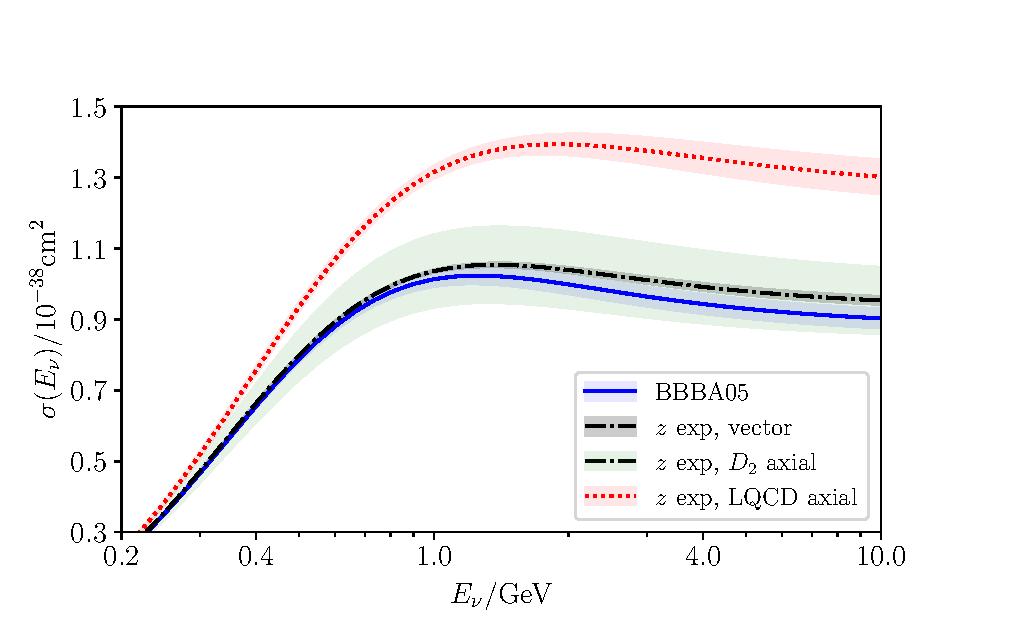
\includegraphics[width=0.7\textwidth]{plots/xsec_comparison-standalone.pdf}\vspace{4pt}
\caption{
 Neutrino cross sections on a free neutron, with their uncertainty bands,
 for various choices of parameterization \new{explained in the bullet list provided in the text}.
 %The curves labeled ``BBBA05'' (blue solid line, Ref.~\cite{Bradford:2006yz})
 %and ``$z$ exp, vector'' (black dot-dashed line, Ref.~\cite{Borah:2020gte}) use the
 %$z$ expansion axial form factor from Ref.~\cite{Meyer:2016oeg},
 %with only the uncertainty from the vector form factors plotted
 %to highlight the tension between the parameterizations shown in Fig.~\ref{fig:protonmagneticff}.
 %The same form factor parameterizations are used for both ``$z$ exp, vector'' and
 %``$z$ exp, D$_{2}$ axial'' (green dot-dashed line)
 %but in the latter case the uncertainty band is taken only from
 %the axial form factor rather than only from the vector form factor.
 %The red dotted line labeled ``$z$ exp, LQCD axial'' is parameterized by
 %the vector form factors of Ref.~\cite{Borah:2020gte} with no uncertainty
 %and the axial form factor with its uncertainty taken from LQCD.
 \label{fig:nucleonxsec}
}
\end{figure}

%\cw{I think these comments are out of place here. They should be removed or worked into the intro or the next section.}
%In the next section, we review the current status of LQCD calculations of the axial form factor.
%We emphasize that LQCD calculations of the electric and magnetic form factors are more mature, but equally important.
%We anticipate, given the state of the field, that within a couple years, we will have a complete error budget for the single nucleon (quasi-) elastic form factors from LQCD.
%
%
%\bigskip\noindent{\color{red}comments below:}
%\begin{description}
%\item[first $z$ exp vector form factor] \cite{Ye:2017gyb}
% - does not use constraints from muonic hydrogen, many more fit parameters
%\item[Vector form factor tensions] \cite{Borah:2020gte}
%\item[Muonic hydrogen review] \cite{Hill:2017wgb}
%\end{description}
%
%\textcolor{red}{[Most focus on axial, but vector is important too]}


% ------------------------------------------------------------------------------
% Lattice QCD
\section{LQCD determinations of the nucleon quasi-elastic form factor\label{sec:lqcd}}
% ------------------------------------------------------------------------------
% LQCD Intro
\subsection{Lattice QCD\label{sec:lqcd_intro}}
Lattice QCD is a discretized version of QCD, formulated in Euclidean spacetime, in which the quark fields live at the sites of the lattice and the gluon fields live on the links between the sites.  These link fields are given by Wilson-lines
\begin{equation}
U_\mu(x) = \exp\left\{i a\int_0^1 dt A_\mu(x +(1-t)a\hat{\mu}) \right\}
    \approx \exp\left\{i a \bar{A}_\mu(x) \right\}\, ,
\end{equation}
where $A_\mu(x)$ is the gluon field, $a$ is the ``lattice spacing'' and $\bar{A}_\mu(x)$ is the average value of $A_\mu(x)$ over the spacetime interval $[x, x+a\hat{\mu}]$.
This parameterization of the gauge fields allows for the construction of a discretized theory which preserves gauge-invariance~\addcite{Wilson}, a key property of gauge theories.
For example, the discretized Dirac operator
\begin{equation}
\bar{\psi}(x)\g_\mu D_\mu \psi(x) \rightarrow
\bar{\psi}(x)\g_\mu\frac{1}{2a}\left[U_\mu(x)\psi(x+a\hat{\mu}) -U^\dagger_\mu(x)\psi(x-a\hat{\mu}) \right]\, ,
\end{equation}
is invariant under gauge transformations,
\begin{align}
&\psi(x)\rightarrow \Omega(x)\psi(x)\, ,&
&U_\mu(x)\rightarrow \Omega(x)U_\mu(x)\Omega^{-1}(x+a\hat{\mu})\, .&
\end{align}


\begin{equation}
\hspace{-1.25in}\Umunu \hspace{-0.65in}
    =U_{\mu\nu}(x)
    =U_\mu(x)U_\nu(x+a\hat{\mu}) U^\dagger_\mu(x+a\hat{\nu}) U^\dagger_\nu(x)
\end{equation}



\bigskip
\begin{itemize}

\item The choice of Euclidean space is to allow Monte Carlo

\item comment on fermion and determinant

\end{itemize}

% ------------------------------------------------------------------------------
% LQCD results
\subsection{Survey of lattice QCD results of $F_A(Q^2)$\label{sec:lqcd_results}}

Citations for $F_A(Q^2)$ references pulled from NME21, no $g_A$-only references:
\begin{description}
\item[NME 21]~\cite{Park:2021ypf}
\item[RQCD 20]~\cite{Bali:2018qus,RQCD:2019jai} %% 63
\item[ETMC 20]~\cite{Alexandrou:2018sjm,Alexandrou:2019brg,Alexandrou:2020okk} %% 54-56
\item[PACS 18 (erratum)]~\cite{Ishikawa:2018rew,Shintani:2018ozy} %% 60-61 (62 proceedings)
\item[PNDME 17]~\cite{Gupta:2017dwj,Gupta:2018qil,Jang:2019vkm,Jang:2019jkn} %% 6-9
\item[CLS 17]~\cite{Hasan:2017wwt,Hasan:2019noy} %% LHPC? 66-67
\end{description}


% ------------------------------------------------------------------------------
% z-expansion
\subsection{Combinding the $z$-expansion with the continuum and chiral extrapolations\label{sec:z_continuum}}



% ------------------------------------------------------------------------------
% Impact
\section{Phenomenological Impact\label{sec:impact}}
Neutrino oscillation experiments measure an event rate, which is the convolution of the flux, cross section and detector efficiency, as a function of some measureable variable. The incoming neutrino energy is not known event by event, and not all outgoing particles are detectable, so quantities such as the energy transfer, or four-momentum transfer, cannot be reconstructed. As neutrino oscillation is a neutrino energy (and distance) dependent phenomenon, experiments attempt to reconstruct it using the kinematics of particles produced when neutrinos interact in their detectors.

T2K, and other experiments with a relatively low energy ($\lessapprox1$ GeV) beam~\cite{Hyper-Kamiokande:2018ofw, MiniBooNE:2020pnu}, attempt to reconstruct the neutrino energy using outgoing lepton momentum, $p_{l}$, and its angle with respect to the incoming beam direction, $\theta_{l}$, assuming two-body quasielastic kinematics with the initial nucleon at rest,
\begin{equation}
E^{\mathrm{rec,\;QE}}_{\nu}\left(p_{l}, \theta_{l}\right) = \frac{2m_f\sqrt{p_{l}^2 + m^2_l} - m_l^2 + m_i^2-m_f^{2}}{2\left(m_f-\sqrt{p_{l}^2 + m^2_l}+p_l \cos\theta_l\right)},
\label{eq:enuqe}
\end{equation}
\noindent where $m_l$ is the mass of the outgoing lepton, $m_{i}$ is the mass of the initial state nucleon, and $m_{f}$ is the mass of the final state nucleon. As this variable assumes quasielastic kinematics, it is applied to a signal sample of CC0$\pi$ events.\footnote{Note that in recent analyses, T2K has included samples including a single charged pion using a modified version of Equation~\ref{eq:enuqe}~\cite{T2K:2017rgv, T2K:2019bcf, T2K:2021xwb}.}%
\begin{marginnote}
\entry{CC0$\pi$}{Events with a muon, no pions or other mesons, and any number of nucleons produced in the final state}
\entry{CCQE}{Charged-current quasielastic}
\entry{CC-2p2h}{Charged-current interactions with two nucleons}
\entry{CC-RES}{Charged-current resonant pion production}
\end{marginnote}%
Events that are not true CCQE events also contribute to the CC0$\pi$ signal, such as CC-2p2h or CC-RES with no visible final-state pion. The two-body approximation in Equation~\ref{eq:enuqe} is a poor approximation of the true neutrino energy, $E_{\nu}^{\mathrm{true}}$, in these cases. Understanding the relative fraction of the different interaction channels is therefore a critical issue for experiments that use Equation~\ref{eq:enuqe}.

\begin{figure}[htbp]
  \centering
  \captionsetup[subfloat]{captionskip=-5pt}
  \subfloat[Near detector]{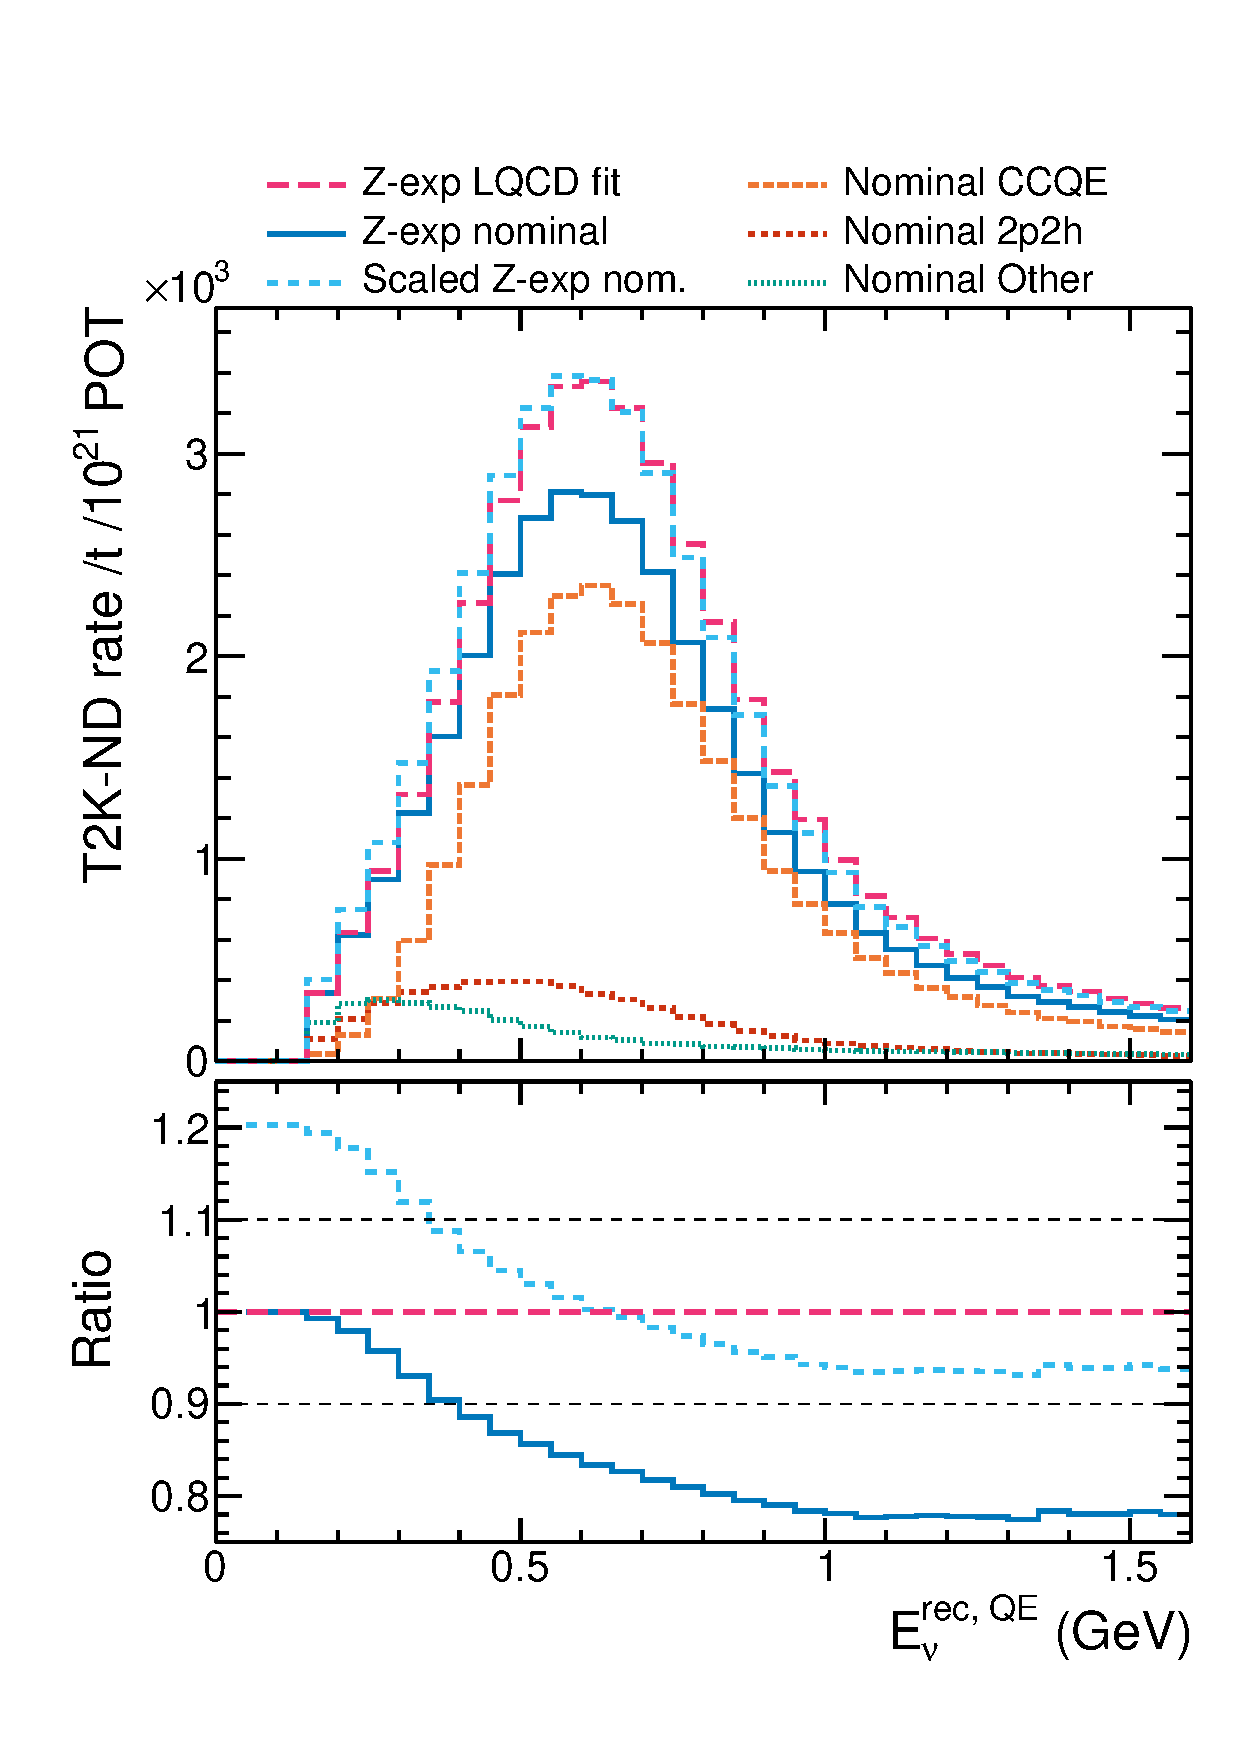
\includegraphics[width=0.3\textwidth]{plots/T2KND_numu_H2O_model_comp.pdf}}\hspace{75pt}
  \subfloat[Far detector] {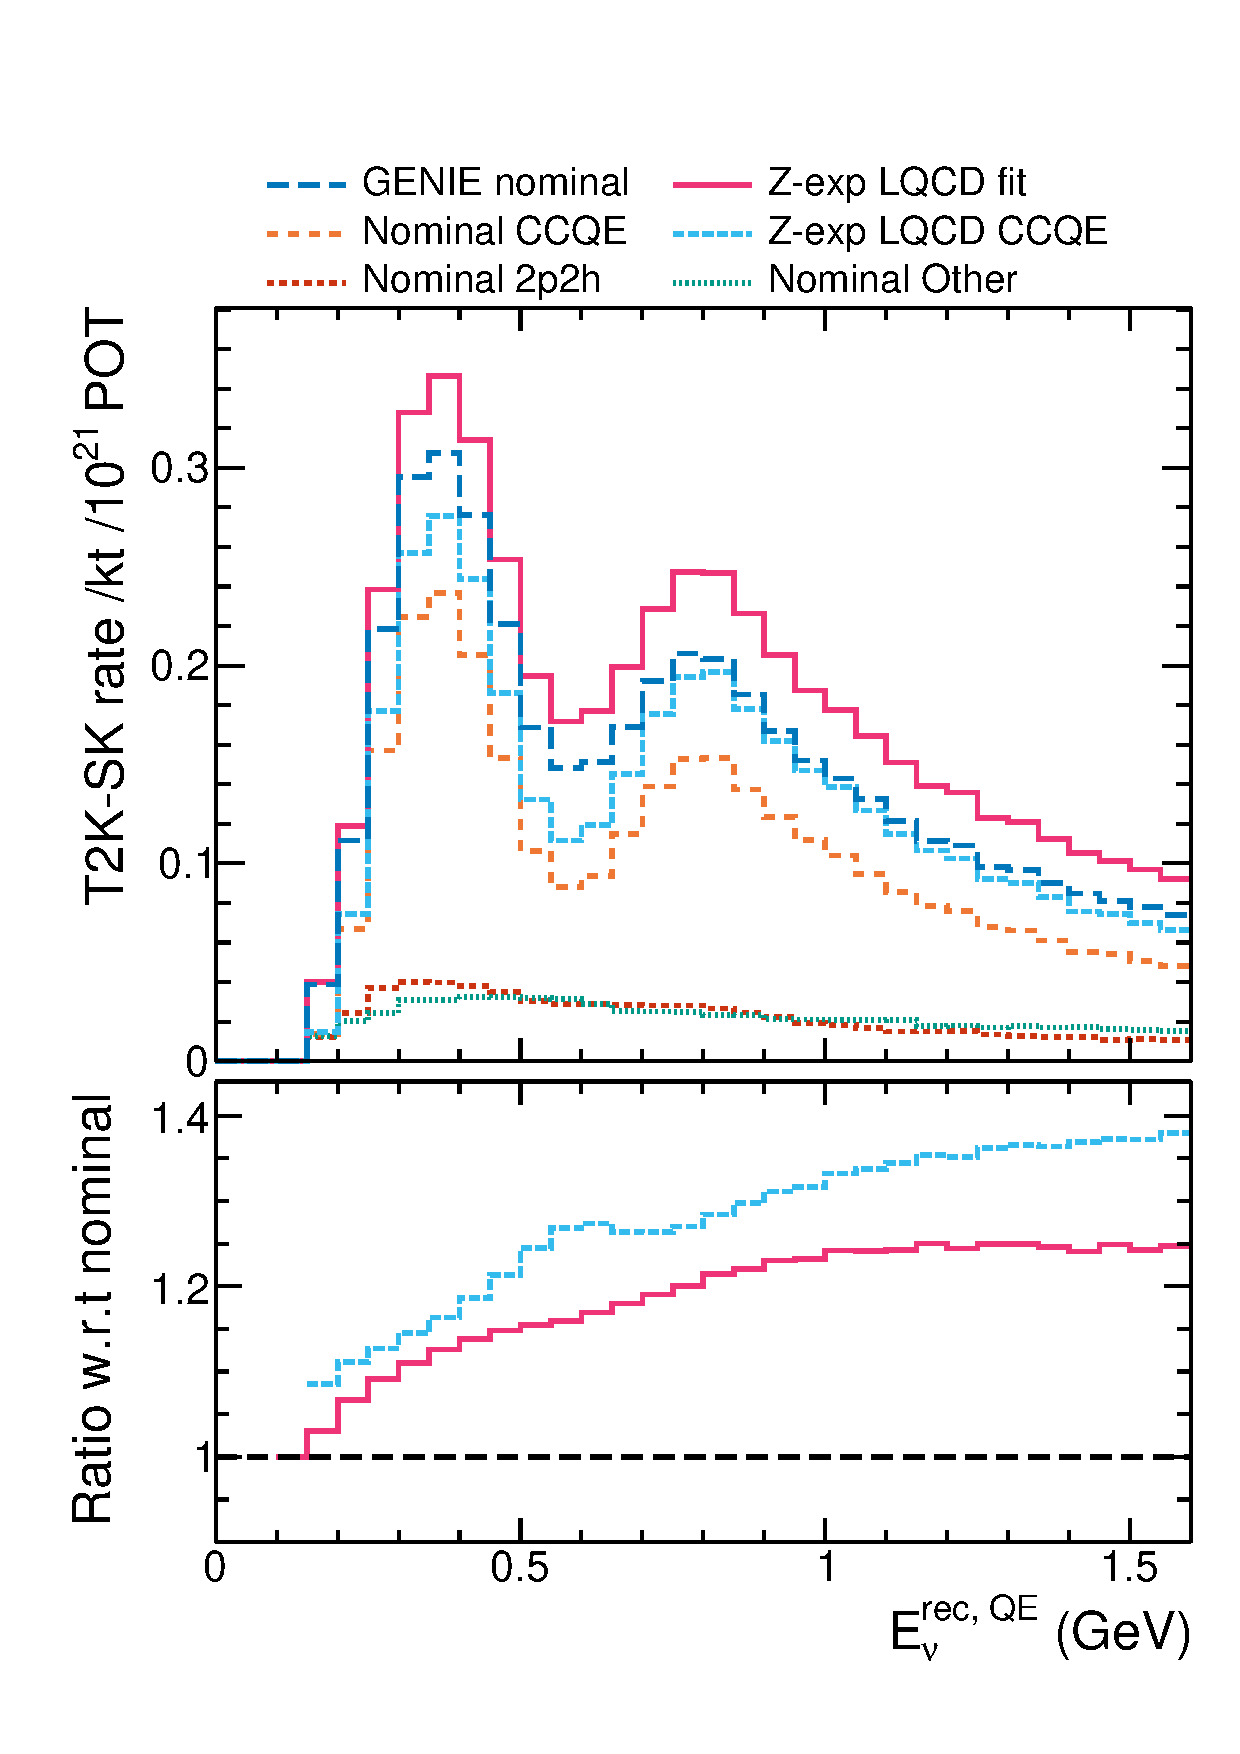
\includegraphics[width=0.3\textwidth]{plots/T2KFD_numu_H2O_osc_model_comp.pdf}}
  \vspace{11pt}
  \caption{The $\nu_{\mu}$--H$_{2}$O CC0$\pi$ event rates per ton (kiloton) per $1\times10^{21}$POT at T2K's near (far) detector site, shown as a function of $E^{\mathrm{rec,\;QE}}_{\nu}$. The GENIE~\cite{Andreopoulos:2009rq, GENIE:2021npt} nominal event rate (blue solid line) is produced using the GENIEv3 10a\_02\_11a tune to nucleon data~\cite{GENIE:2021zuu} and the T2K flux~\cite{T2K:2012bge}, and the CCQE (orange dashed line), CC-2p2h (red short dashed line) and CC-other (green dotted line), here meaning all events that are note CCQE or CC-2p2h, contributions are shown. The oscillated flux is calculated using the best fit NuFit5.0 oscillation parameters in normal ordering~\cite{Esteban:2020cvm, nufitweb}. Additionally, an alternative GENIE model is shown, where the only change is to use the $z$ expansion model of the axial form factor, with parameters tuned to LQCD results from the CalLat collaboration, as described in Section~\ref{sec:callatdata}. Additionally, the ratio of the modified to nominal GENIE models is shown.}
  \label{fig:t2k_impact}
\end{figure}
Figure~\ref{fig:t2k_impact} shows the $\nu_{\mu}$--H$_{2}$O CC0$\pi$ event rate expected at the T2K near and far detectors for a fixed exposure, shown as a function of $E^{\mathrm{rec,\;QE}}_{\nu}\left(p_{l}, \theta_{l}\right)$, with and without modifications to the axial form factor. The nominal GENIEv3 10a\_02\_11a model~\cite{Andreopoulos:2009rq, GENIE:2021npt} uses a dipole axial form factor with $M_{\mathrm{A}} = 0.941$%
\begin{marginnote}
 \entry{$M_{\mathrm{A}}$}{dipole axial mass parameter}
\end{marginnote}%
 GeV obtained through a fit to bubble chamber data~\cite{GENIE:2021zuu}. The alternative model shown differs only in the use of the $z$ expansion model for the axial form factor, with parameters tuned to the LQCD results from the CalLat collaboration described in Section~\ref{sec:callatdata}. One obvious observation to be made from Figure~\ref{fig:t2k_impact} is that the CCQE events which the axial form factor is relevant for clearly make up the majority of T2K's CC0$\pi$ sample, in both the oscillated and unoscillated fluxes. It is also clear that the tuned LQCD values has significant effect on the total expected event rate in both cases, on the order of 20\%.

Also clear from Figure~\ref{fig:t2k_impact} is that the change in the total, or CCQE-contributed event rates is not purely a normalization change, and is different for the near and far detector spectra. In the T2K oscillation analysis, the near detector data is used to constrain the cross section model, to reduce the uncertainty at the far detector and on the measured oscillation parameters. If there is insufficient freedom in the cross section model to account for this change to the CCQE model, other parts of the model may well be distorted to ensure good agreement with the near detector data. However, this can introduce biases at the far detector, as the different interaction types that contribute to the CC0$\pi$ samples shown in Figure~\ref{fig:t2k_impact} have very different $E_{\nu}^{\mathrm{true}}$ --- $E^{\mathrm{rec,\;QE}}_{\nu}$ relationships. So if other components of the model are distorted to fit the unoscillated near detector event rate, that same {\it effective} change is not in general expected to extrapolate to the far detector spectrum correctly.

Experiments with higher neutrino beam energies typically do not limit their analyses to CC0$\pi$ events or use Equation~\ref{eq:enuqe} for reconstructing the neutrino energy. Instead, they use all charged-current events (CC-inclusive), and reconstruct the neutrino energy through a combination of particle identification and tracking, and calorimetry. For an ideal detector, with no tracking threshold on protons, charged pions or electromagnetic activity, this can be expressed as,
\begin{equation}
E_{\nu}^{\mathrm{rec,\;had}} = E_{l} + \Sigma_{p} E_{\mathrm{kin}} + \Sigma_{\pi^{\pm}, \pi^{0}, \gamma} E_{\mathrm{total}},
\label{eq:enuhad}
\end{equation}
\noindent where $E_{l}$ is the energy of the outgoing charged lepton. The $E_{\nu}^{\mathrm{true}}$ --- $E_{\nu}^{\mathrm{rec,\;had}}$ smearing in this idealized case is due to missing kinetic energy lost to neutrons, and initial state nuclear effects (e.g., nucleons are not at rest inside the nucleus). Real detectors have tracking thresholds below which charged particles cannot be reconstructed, which results in additional smearing due to missing the masses of charged pions, although some energy lost to neutrons may be recovered.

\begin{figure}[htbp]
  \centering
  \subfloat[ND]{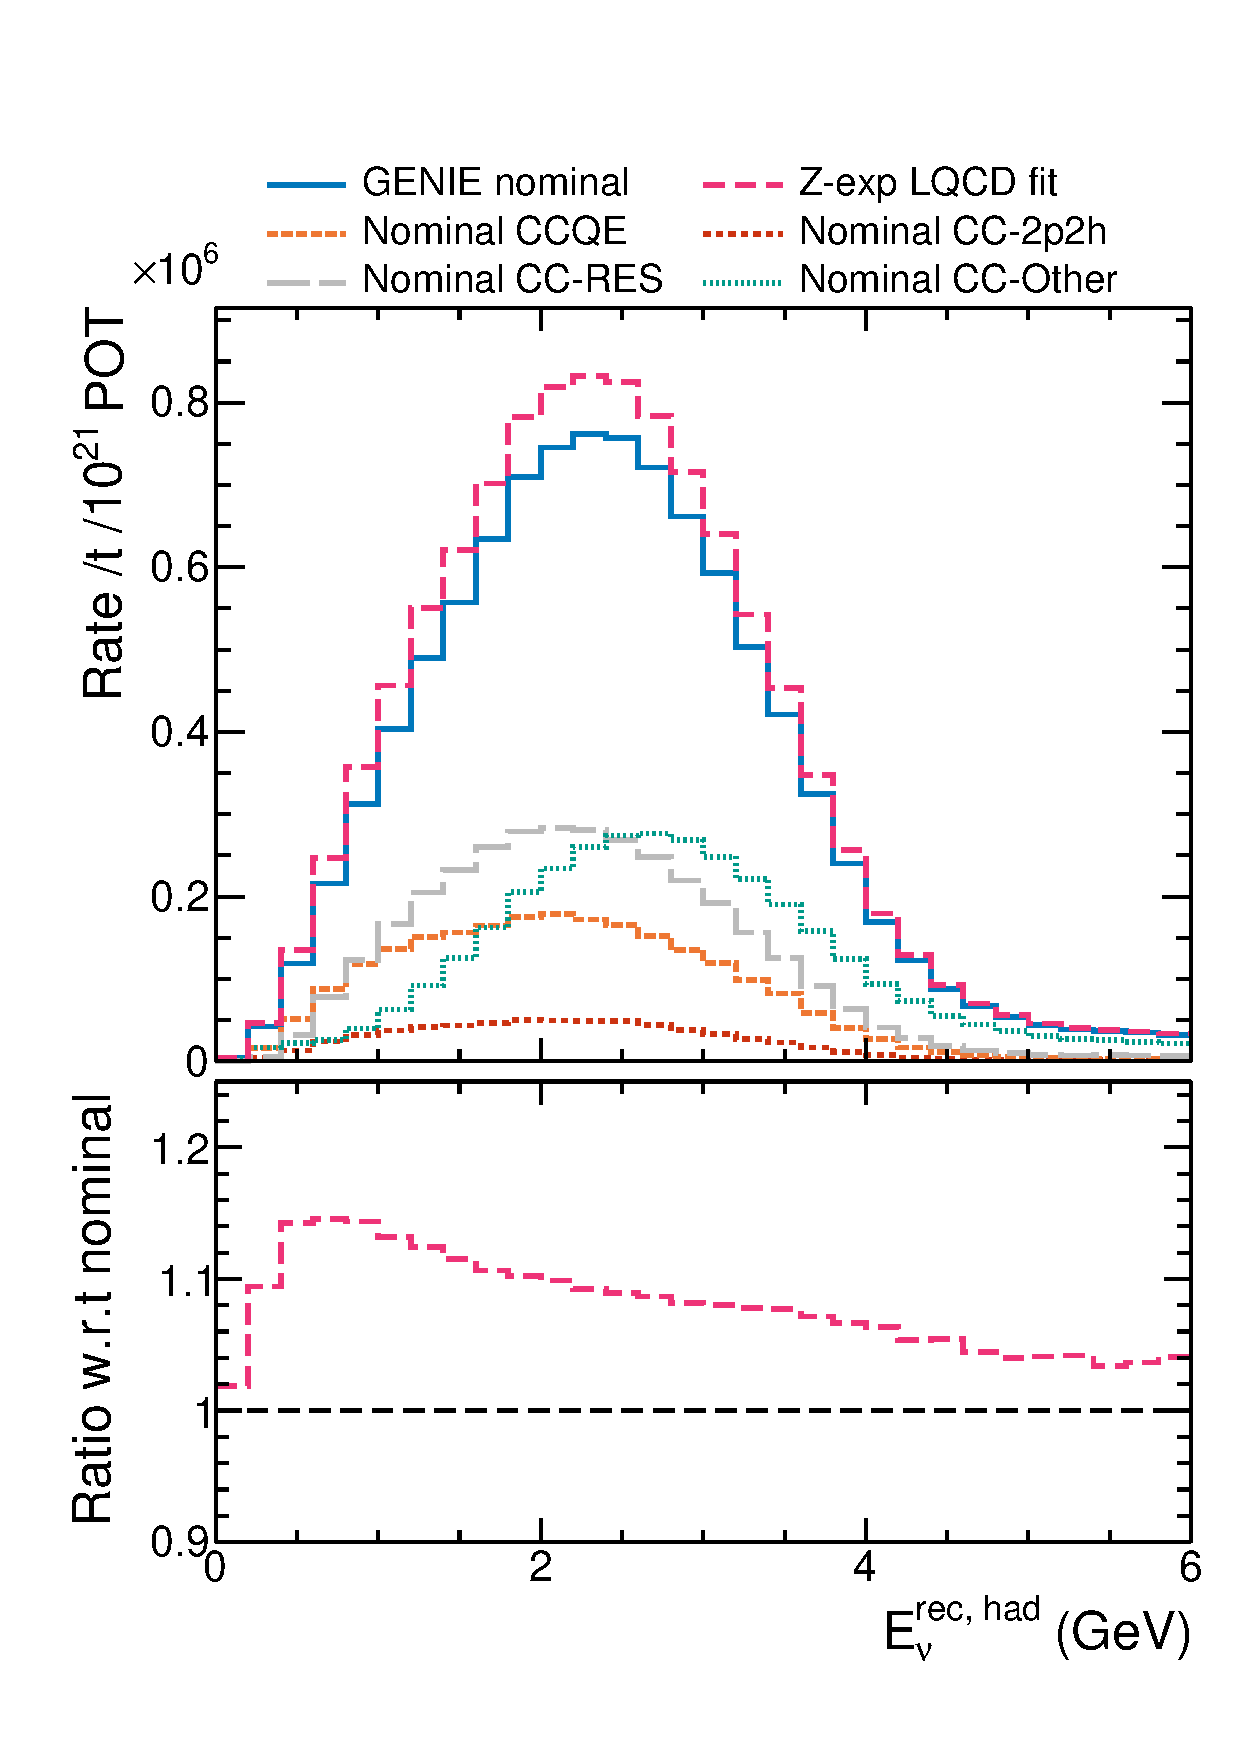
\includegraphics[width=0.3\textwidth]{plots/DUNE_numu_Ar40_breakdown.pdf}}\hspace{75pt}
  \subfloat[FD]{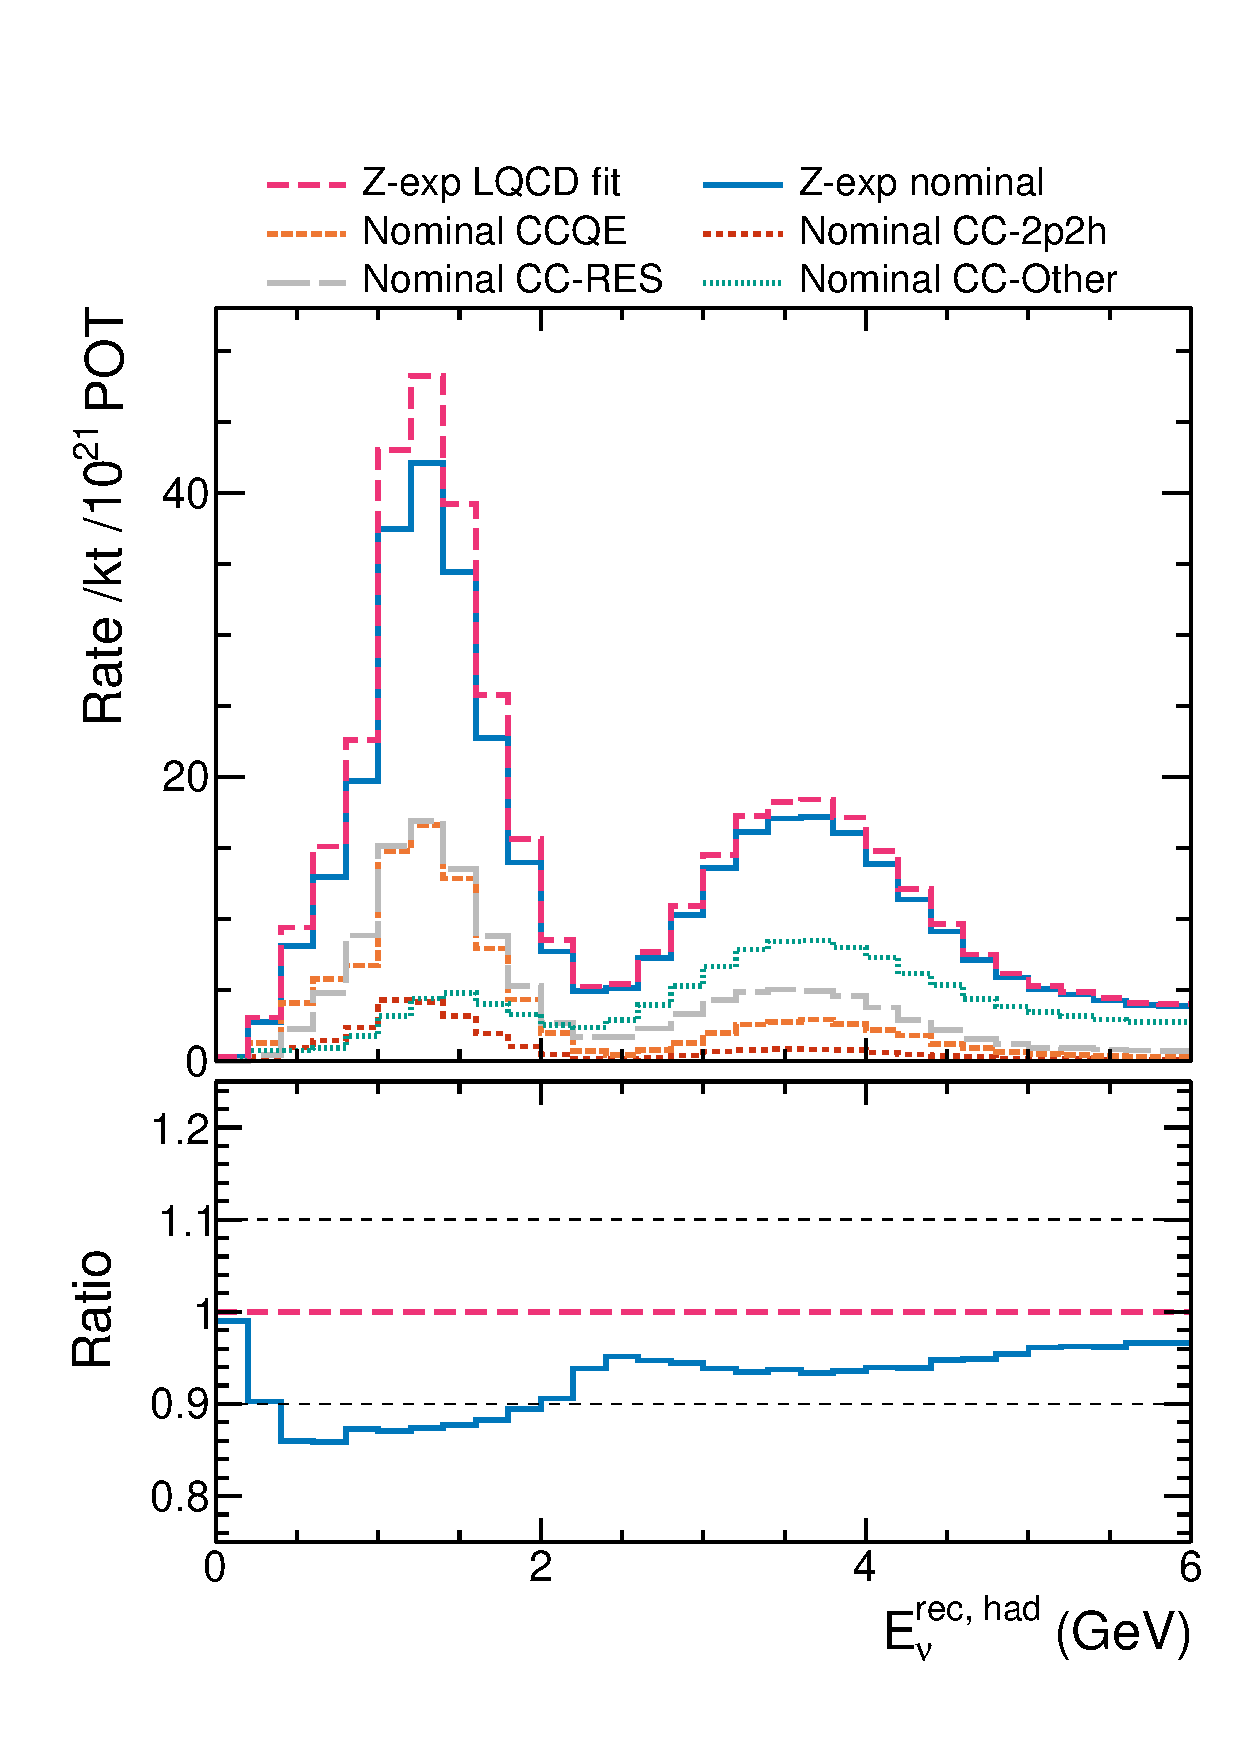
\includegraphics[width=0.3\textwidth]{plots/DUNE_osc_numu_Ar40_breakdown.pdf}}
  \vspace{11pt}
  \caption{The $\nu_{\mu}$--$^{40}$Ar CC-inclusive event rates per ton (kiloton) per $1\times10^{21}$POT at DUNE's near (far) detector site, shown as a function of $E^{\mathrm{rec,\;had}}_{\nu}$. The GENIE~\cite{Andreopoulos:2009rq, GENIE:2021npt} nominal event rate (blue solid line) is produced using the GENIEv3 10a\_02\_11a tune to nucleon data~\cite{GENIE:2021zuu} and the DUNE flux~\cite{Abi:2020evt}, and the CCQE (orange dashed line), CC-2p2h (red short dashed line), CC-RES (long-dashed gray line) and CC-other (green dotted line), here meaning all events that are not CCQE, CC-2p2h or CC-RES, contributions are shown. The oscillated flux is calculated using the best fit NuFit5.0 oscillation parameters in normal ordering~\cite{Esteban:2020cvm, nufitweb}. Additionally, an alternative GENIE model is shown, where the only change is to use the $z$ expansion model of the axial form factor, with parameters tuned to LQCD results from the CalLat collaboration, as described in Section~\ref{sec:callatdata}. Additionally, the ratio of the modified to nominal GENIE models is shown.}
  \label{fig:dune_impact}
\end{figure}
Figure~\ref{fig:dune_impact} shows the $\nu_{\mu}$--$^{40}$Ar CC-inclusive event rates per ton (kiloton) per $1\times10^{21}$POT at DUNE's near (far) detector site, shown as a function of $E^{\mathrm{rec,\;had}}_{\nu}$, with and without modifications to the axial form factor. At this higher neutrino beam energy (with $E_{\nu}^{\mathrm{peak}} \approxeq 2.5$ GeV), CCQE events still make up a sizeable, $\approx$30\%, fraction of the total events. The modification to the axial form factor based on the LQCD results from the CalLat collaboration described in Section~\ref{sec:callatdata} has an approximately 10\% effect to the total predicted event rate at both the near and far detectors, with different shape dependence, as in the T2K case. Despite the different neutrino energy reconstruction methods used by DUNE and T2K, the same arguments about potential bias due to model-dependence apply when there are differences in the effect of an out-of-model change between near and far detectors.

The issue of how to assign strength between the CCQE and CC-2p2h channels has been a major focus for neutrino oscillation experiments over the past decade. Experimental data from a large number of experiments has found disagreements on the 10--30\% level between model predictions and data in the CC$0\pi$ channel~\cite{garvey_review_2014, Mosel:2016cwa, NuSTEC:2017hzk, Katori:2016yel, ParticleDataGroup:2020ssz}, prompting development of {\it ad hoc} systematic uncertainties and empirical model tunings by individual experiments, with a tendancy has been to soak up model-data discrepancies into the CC-2p2h channel. These are major contributors to the final uncertainties on key oscillation parameter measurements and projected sensitivities~\cite{T2K:2019bcf, DUNE:2020jqi, T2K:2021xwb, NOvA:2021nfi, DUNE:2021mtg}. It is therefore very significant that the LQCD results shown in Figures~\ref{fig:t2k_impact} and~\ref{fig:dune_impact} suggest that an increase to the strength of the CCQE contribution on the order of 20\% is necessary.



% ------------------------------------------------------------------------------
% Future
\section{Future Improvements\label{sec:future}}
{\color{red}items to comment on}
\begin{itemize}
\item won't be performing precision calculations at 2-3 fm
\item variational with pi-N operators
\item this enables Breit-Frame and improved single-nucleon
\item domain-decomposed idea of Giusti et al
\end{itemize}


Precise nucleon form factors for (quasi)elastic scattering are of the most immediate concern
 for neutrino oscillation experiments and simultaneously one of the easiest
 targets for LQCD in regards to nucleon interactions.
\new{Higher energy transfer processes also play a sub-dominant role for T2K (and the future
Hyper-K) experiments, and a major role in the DUNE experiment which has a higher energy neutrino
flux, as can be seen in Figures~\ref{fig:t2k_impact} and~\ref{fig:dune_impact}, respectively.}
These higher energy transfers can access other fundamentally different interaction topologies,
 such as resonant or nonresonant pion production mechanisms,
 nuclear responses with correlated nucleon pairs,
 or scattering off partons within nucleons.
In principle, all of these interaction mechanisms are accessible to LQCD,
 though with varying degrees of difficulty.
Given the discrepancy between lattice axial form factor data and experimental constraints,
 it is not unreasonable to expect other interaction mechanisms have similar discrepancies
 between theory and observation.
These interaction types are more challenging to extract or even inaccessible to
 experimental measurements.
Appeals to model assumptions may give some handle for missing quantities,
 but are also subject to unquantifiable systematic effects.

Calculations that access the combined resonant and nonresonant scattering amplitudes
 are the most similar to those of elastic scattering,
 where a current induces a transition of the nucleon to a multiparticle final state.
Only stable final states, such as nucleon-pion states or other multiparticle states,
 are obtained as eigenstates of the Hamiltonian.
Resonance properties are indirectly probed by converting the observed spectrum,
 with its power-law finite volume corrections, to a scattering phase shift in infinite volume.
These power-law finite volume corrections are in contrast with exponentially-damped
 corrections obtained for single-particle states.
The multiparticle states make up a dense spectrum that arises from
 states where individual hadrons move with different discrete lattice momenta.

The main difficulties in these calculations stem the challenges of extracting
 information about many excited states rather than a single ground state.
Empirical evidence from dedicated computations demonstrates that these multiparticle states
 are in practice difficult to quantify without interpolating operators constructed to
 closely resemble the states they are intended to identify,
 both in the number of quarks and antiquarks and also the individual
 momenta of the quark-level components~\textcolor{red}{[cite JLab]}.
The necessary interpolating operators for extracting multiparticle states often have
 unfavorable combinatoric factors multiplying the number of terms to account for
 permutations of quark lines, changing momenta, varying time ranges, or the like.
Some form of approximate all-to-all method is likely necessary
 to compute amplitudes of nucleon resonant and nonresonant transitions
 to states with pions.

The aforementioned issues are, at least in part, circumvented by applying approximate
 all-to-all techniques, for instance distillation~\textcolor{red}{[citations]}.
Though the overhead for these methods is large,
 these techniques enable sophisticated calculations with large bases
 of interpolating operators including multiparticle interpolators.
Using an all-to-all method specifically avoids the need to produce sequential
 quark propagator inversions that are used in traditional three-point correlator functions,
 which are the source of many unfavorable combinatoric factors and are
 costly when enumerating all possible quark line combinations.
Though the lowest resonances will be accessible with these techniques,
 the higher-mass resonances will be more technically difficult
 due to the increased density of states with the energy transfers involved.
Using these propagator data, a calculation of the Roper resonance contribution
 has the secondary consequence of offering a handle on removing excited
 state contamination from a calculation of the quasielastic form factors.
\textcolor{red}{[summarizing statement or two about current status]}

To access higher resonance states in the so-called shallow inelastic scattering (SIS) regime,
 lattice calculations will likely be more successful using other methods
 that access the inclusive nucleon scattering amplitude to hadronic states.
A four-point function calculation on the lattice can obtain a discrete sampling
 of the scattering amplitude as a function of the center-of-mass energy,
 convolved with weights that are exponential in the energy and time separation.
Applying an inverse transformation to obtain the scattering amplitude
 is an ill-posed problem, but initial calculations using techniques
 such as Backus-Gilbert or moments have shown promise.
\textcolor{red}{[more detail, references, check wording]}

Calculations of two-nucleon matrix elements provide key insights
 about the correlations between nucleons inside of a nuclear medium,
 a vital ingredient for construction of an effective theory
 of neutrino interactions with nuclear targets.
%% heavier than physical Mpi => NPLQCD/HALQCD controversy
First efforts have been made to compute deuteron and dineutron scattering phase shifts
 at unphysically heavy pion masses.
There is some controversy about whether the deuteron forms a
 bound state at these higher pion masses.~\textcolor{red}{[citations, more content]}.

%% gA(Q2) on D2 and nuclear ET
Future calculations of matrix elements for currents inserted between
 two-nucleon states could provide direct information about the LEC inputs to nuclear
 models~\cite{Drischler:2019xuo}
 or by providing direct comparisons of neutrino interaction matrix elements in deuterium.
\textcolor{red}{[more detail needed on ET LECs]}
%% overlap of energy scales of NN vs NNpi
\textcolor{red}{[the following is likely too much detail]}
Deuterium corrections from nuclear models were assumed to be strong only at low momentum transfer
 and energy-independent in the reanalysis of deuterium bubble chamber data~\cite{Meyer:2016oeg},
 despite the inability of these corrections to account for the theory-data discrepancies.
A direct LQCD computation of these effects would isolate the effect,
 either by definitively attributing the discrepancy to deuterium effects
 or by implicating the other systematics corrections.



% ------------------------------------------------------------------------------
% Conclusions
\section{Conclusions\label{sec:conclusions}}
LQCD collaborations are able to produce consistent results for benchmark quantities such as $g_{\mathrm{A}}$ with percent level systematic uncertainties, which are in excellent agreement with experimental data.
These results introduce the exciting possibility of LQCD calculations to tackle other quantities for which are not easily experimentally accessible, or for which tensions between measurements, or competing models, exist.
In this review we discussed using LQCD to calculate nucleon form factors as a function of momentum transfer, which are of particular interest to the few-GeV neutrino experimental program.
Important tensions exist in current parameterizations of the vector form factors, but here we focused on the axial form factor, $F_{\mathrm{A}}(Q^2)$, which is of primary importance because current parameterizations of it are simplistic and rely on a handful of low-statistics neutrino--H$_2$ and neutrino--D$_2$ bubble chamber measurements.
It cannot be cleanly measured with existing experiments which use heavier nuclear targets for safety reasons and to increase the event rate, so LQCD offers a novel path to this important quantity.
We have compared $F_{\mathrm{A}}(Q^2)$ calculations from a variety of different LQCD collaborations using different approaches and techniques, and shown them to be in good agreement with each other, but crucially, in poor agreement with the simple dipole model tuned to historic neutrino--D$_2$ data currently relied upon.
Assuming that no systematic effects affecting all of the LQCD calculations are uncovered, this suggests a significant increase of approximately 20\% to the strength of the CCQE scattering channel that dominates the neutrino scattering cross section for $E_{\nu} \lesssim 1$ GeV.
We have demonstrated that these results produce a significant change in the predicted neutrino event spectra for T2K (which has similar considerations to Hyper-K) and DUNE experiments.
Determining the impact on oscillation results would require a full analysis performed by each experimental collaboration, but it is clear that LQCD results for $F_{\mathrm{A}}(Q^2)$ may offer a valuable insight that can clarify aspects of the complex neutrino interaction modeling problem these experiments face.
We additionally discussed a number of ways in which current calculations can be improved and validated, to increase confidence that the LQCD results are not subject to an uncontrolled systematic uncertainty, and to reduce systematics.
Finally, we discussed a number of other quantities which are important to neutrino oscillation experiments in the few-GeV energy regime which LQCD can provide data for, for which there are no experimental solutions, including resonant pion production at higher energy transfers, which is of particular interest to the DUNE experimental program, and insights into nucleon-nucleon correlations.
These possibilities would all work to break degeneracies and overcome experimental challenges that affect current neutrino-nucleus interaction modelling efforts.

%% \cw{Added some very rough bullet points below}
%% \begin{itemize}
%% \item LQCD collaborations are now producing consistent results for a number of benchmark quantities, which are in agreement with experimental data.
%% \item Able to calculate nucleon form factors with current techniques. Results for FA from different collaborations using different approaches are in agreement --- unlikely to be a common missing systematic uncertainty
%% \item LQCD FA results differ from experimental measurements from old nu-H and nu-D bubble chambers. These are important quantities for current neutrino oscillation experiments, but cannot be measured cleanly as all modern neutrino scattering and oscillation experiments use heavy nuclear targets for safety reasons and to increase the event rate.
%% \item We have demonstrated how these results produce a significant change for T2K (Hyper-K) and DUNE experiments. Determining the impact on oscillation results would require a full oscillation analysis performed by each experimental collaboration, but clear that LQCD can reduce uncertainties.
%% \item There are a number of other quantities which are important to neutrino oscillation experiments in the few-GeV energy regime which LQCD can provide data for, for which there are no experimental solutions.
%% \end{itemize}



%Disclosure
\section*{DISCLOSURE STATEMENT}
The authors are not aware of any affiliations, memberships, funding, or financial holdings that might be perceived as affecting the objectivity of this review.

% Acknowledgements
\section*{ACKNOWLEDGMENTS}
This work was supported by the Director, Office of Science, Office of Basic Energy Sciences, of the U.S. Department of Energy under Contract No. DE-AC02-05CH11231.

%% Supposedly, we should always include these things as LBNL employees: https://commons.lbl.gov/display/rpm2/Scientific+and+Technical+Publications+Requirements#myId--1898802862 (section D.2)
%This document was prepared as an account of work sponsored by the United States Government. While this document is believed to contain correct information, neither the United States Government nor any agency thereof, nor the Regents of the University of California, nor any of their employees, makes any warranty, express or implied, or assumes any legal responsibility for the accuracy, completeness, or usefulness of any information, apparatus, product, or process disclosed, or represents that its use would not infringe privately owned rights. Reference herein to any specific commercial product, process, or service by its trade name, trademark, manufacturer, or otherwise, does not necessarily constitute or imply its endorsement, recommendation, or favoring by the United States Government or any agency thereof, or the Regents of the University of California. The views and opinions of authors expressed herein do not necessarily state or reflect those of the United States Government or any agency thereof or the Regents of the University of California.

%This manuscript has been authored by an author at Lawrence Berkeley National Laboratory under Contract No. DE-AC02-05CH11231 with the U.S. Department of Energy. The U.S. Government retains, and the publisher, by accepting the article for publication, acknowledges, that the U.S. Government retains a non-exclusive, paid-up, irrevocable, world-wide license to publish or reproduce the published form of this manuscript, or allow others to do so, for U.S. Government purposes.

% References
\bibliography{AR_review.bib}
\bibliographystyle{ar-style5}
%ArXiv references may be formatted as follows, in the Literature Cited section: “1. Author A, Author B. arXiv:XXXX.XXXX [hep-ph] (2017)”

\end{document}
